\section{Bài toán phối hợp đẩy vật }
\label{sec:pushing}
Bài toán thao tác vật thể (object manipulation) đối với hệ thống đa robot là việc triển khai một bầy robot di động cùng tham gia thao tác và điều khiển chuyển động của một vật thể trong một môi trường cụ thể, ví dụ như là trên một mặt phẳng 2D. Các robot có thể tương tác trực tiếp hoặc gián tiếp với vật thể thông qua các cơ cấu chấp hành mà nó sở hữu làm cho vật thể di chuyển theo quỹ đạo mong muốn hoặc đạt đến vị trí mục tiêu, đồng thời đảm bảo chuyển động diễn ra ổn định, không mất tiếp xúc và không gây xoay lệch ngoài ý muốn. Có thể chia thành hai loại hình tương tác chính là cầm nắm (prehensile) - truyền lực thông qua tiếp xúc kẹp, bám hoặc hình học khoá cứng (form-closure) và không cầm nắm (non-prehensile) - chỉ truyền lực qua tiếp xúc bên ngoài và bị chi phối mạnh mẽ bởi ma sát, vị trí tiếp xúc và hình học của vật. Trong đó thì phương pháp đẩy (pushing) là một trong những phương pháp phổ biến nhất thuộc nhóm không cầm nắm, cho phép robot tác dụng lực đẩy vào bề mặt bên ngoài của vật thể để sinh ra lực và mô men, từ đó điều khiển chuyển động của vật thể và không cần phải giữ chặt lấy vật. Điều này khiến cho việc thiết kế cơ khí của robot trở nên dễ dàng hơn, khi thiết kế các cơ cấu chấp hành phục vụ cho việc tạo ra và duy trì lực đẩy thường đơn giản và dễ kiểm soát hơn so với cơ các cơ cấu loại cầm nắm như tay gắp, giác hút rất nhiều. Điều này mang lại lợi thế rất lớn, đặc biệt cho hệ thống đa robot khi mà nó làm giảm chi phí chế tạo, tính toán cục bộ trên mỗi đơn vị đi đáng kể.
\begin{figure}[H]
    \centering
    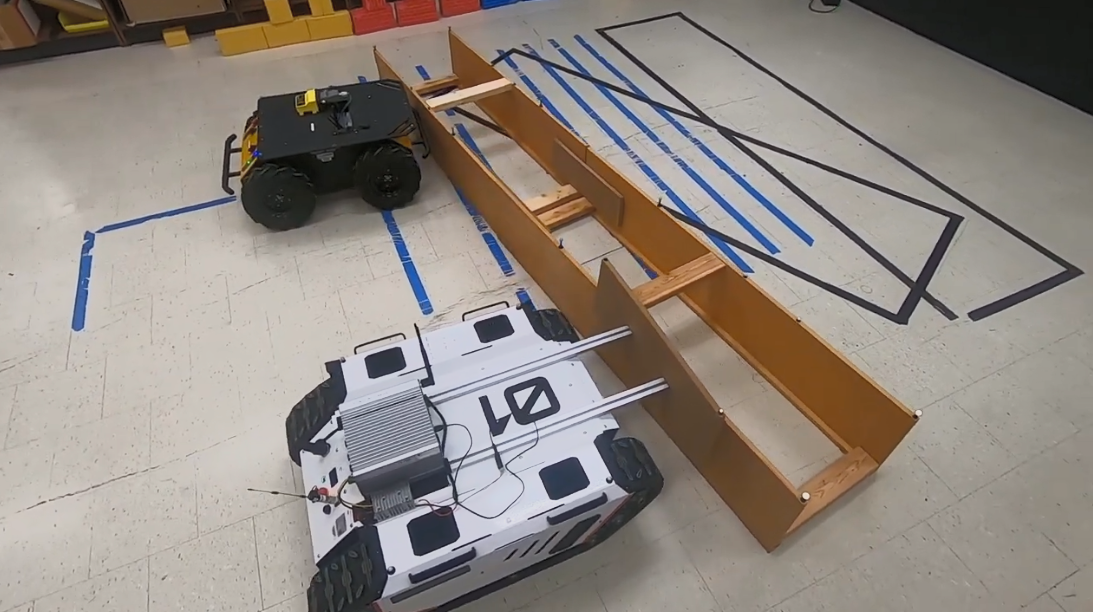
\includegraphics[scale=0.6]{chapter1/image/pushing_ex.png}
    \caption{Hai robot đang phối hợp đẩy vật}
    \label{fig:ex}
\end{figure}

Trong lĩnh bực thao tác vật thể nói chung và đẩy vật nói riêng của hệ thống đa robot, bài toán đầu tiên và cũng quan trọng nhất cần được giải quyết đó chính là xác định được các đội hình phù hợp để hệ robot bám theo và thay đổi nhằm thích ứng với yêu cầu điều khiển. Đội hình (formation) đóng vai trò như cấu trúc tổ chức của các robot, quy định vị trí tiếp xúc, hướng đẩy và sự phân bổ lực giữa từng robot trong quá trình di chuyển vật. Do đặc tính của thao tác non-prehensile, vật có thể dễ dàng bị xoay lệch hoặc mất ổn định nếu vị trí các robot không được bố trí hợp lý. Mỗi phương pháp xây dựng cấu hình khác nhau sẽ tương ứng với một chiến thuật điều khiển khác nhau, nhằm đảm bảo vật đạt được chuyển động mong muốn. Chiến thuật đẩy đóng vai trò như bộ điều khiển của các robot, quyết định xem tổng hợp hành vi của các đơn vị có đạt được đến mục tiêu toàn cục không.    

